\chapter{ZENER REGULATOR WITH SERIES PASS TRANSISTOR}

\subsection*{AIM}
To design and implement a zener diode regulator with series pass transistor and to plod the line regulation characteristics.

\subsection*{DESIGN AND CIRCUIT DIAGRAM}
\paragraph{}
Zener diode maintains a constant voltage acroos its terminals when reverse biased and the applied volatage is above the reverse breakdown voltage of the diode.

The circuit diagram for implementing a series pass transistor zener diode regulator is shown in Figure \ref{zenerregulatorckt}.



\subsection*{PROCEDURE}

\subsubsection{Launch eSim}

\paragraph{}
 Launching eSim will take you to the dialog box. It asks for the default workspace. Browse the folders and set the wokspace location. It will end up in the eSim window shown in Figure \ref{LaunchWindow}.
 
\begin{figure}[H]
\centering
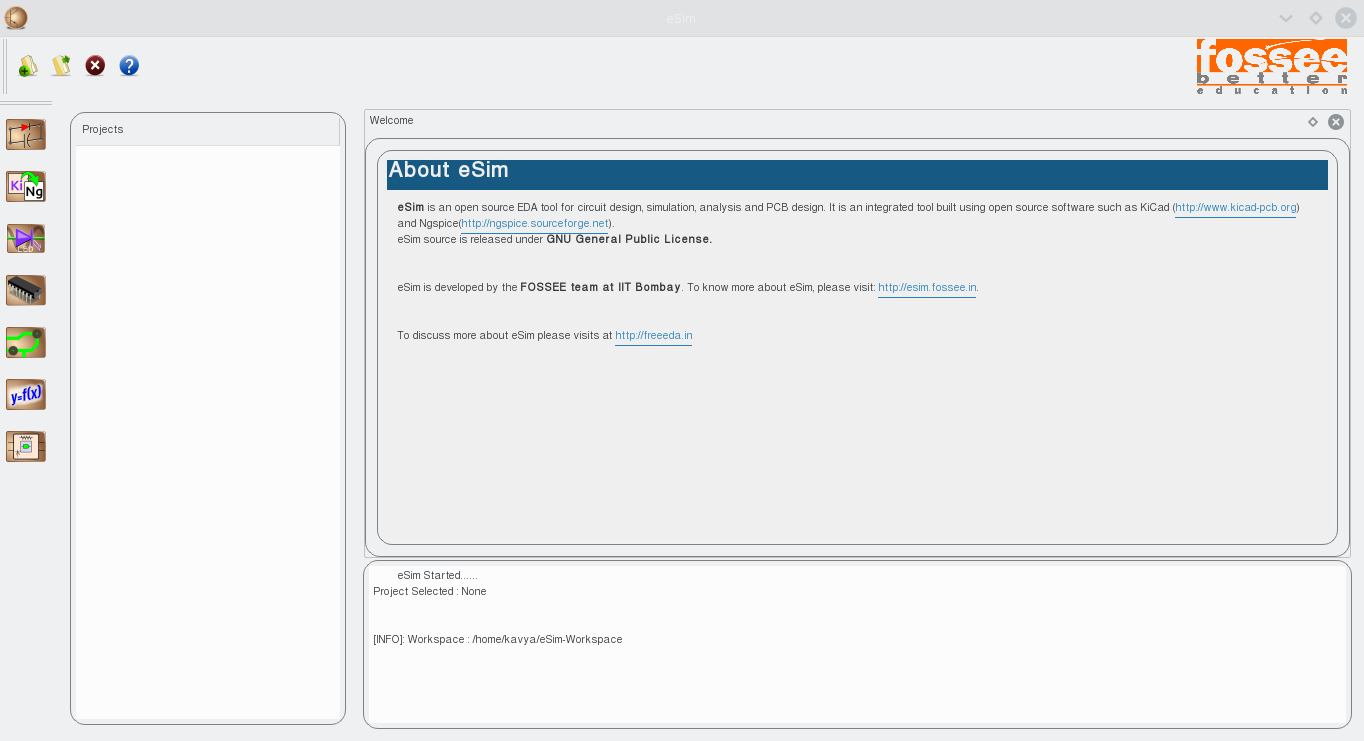
\includegraphics[width=0.8\textwidth]{LaunchWindow.png}
\caption{Launching eSim will take you to this window}
\label{LaunchWindow}
\end{figure}

\subsubsection{Create a New Project}

\paragraph{ } The new project is created by clicking the New icon on the
menubar. Give the name of the project ,'ZenerRegulator' in the pop up window as shown in Figure.\ref{newproject}. 
\begin{figure}[H]
\centering
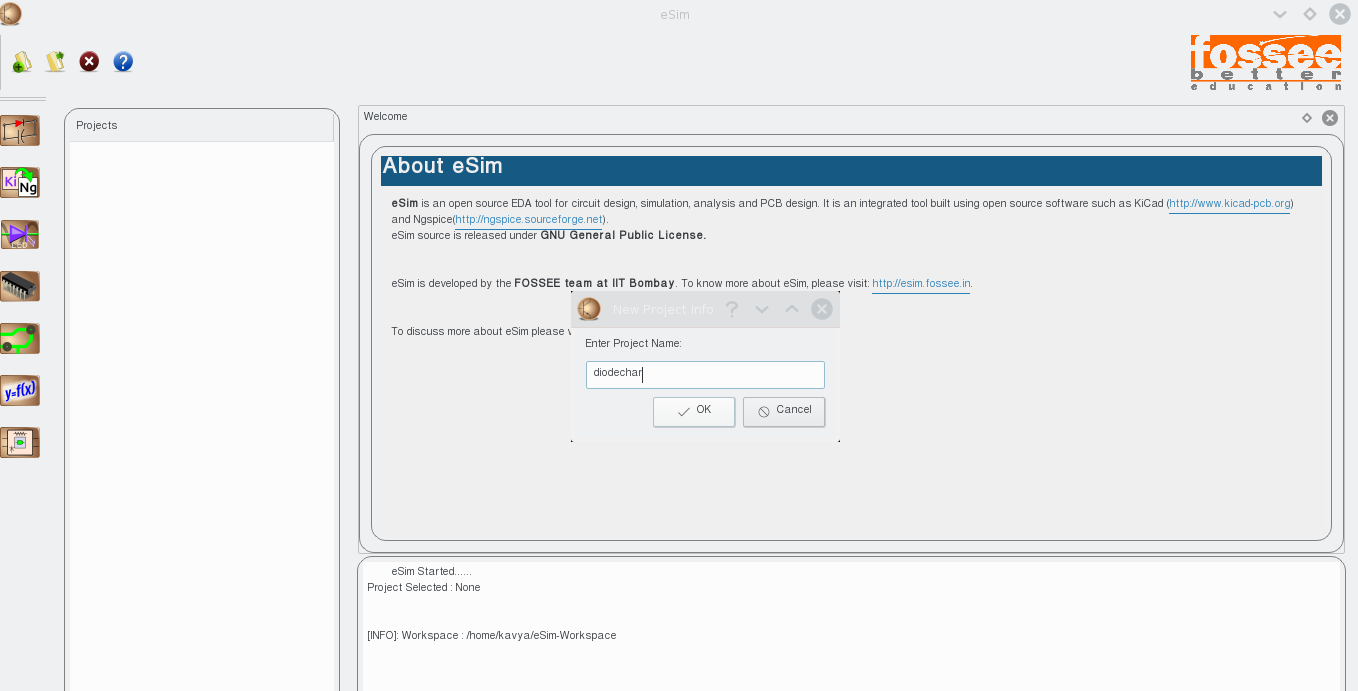
\includegraphics[width=\textwidth]{newproject.png}
\caption{Creating new project}
\label{newproject}
\end{figure}

\subsubsection{Create the Schematic}

\paragraph{}  To create the schematic, click the very first icon of the
left toolbar as shown in the Figure \ref{newschematic} .This will open KiCad Eeschema.


\begin{figure}[H]
\centering
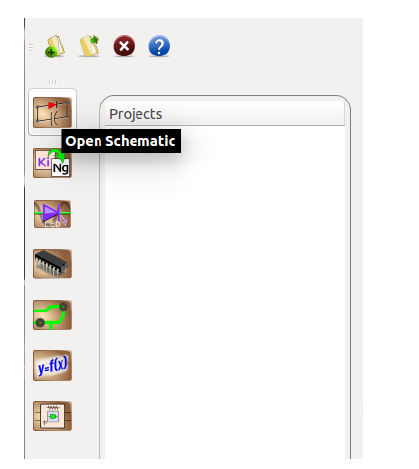
\includegraphics[width=0.5\textwidth, height=6cm]{newschematic.png}
\caption{Creating new schematic diagram}
\label{newschematic}
\end{figure}

To create a schematic in KiCad, we need to place the required components. See Figure \ref{kicad}.  Figure \ref{placecomponent}
shows the icon on the right toolbar which opens the component library. After all the required components of the simple RC circuit are placed, wiring is
done using the Place Wire option as shown in the Figure \ref{placewire}. Scroll up and down for zooming in and out.

\begin{figure}[H]
\centering
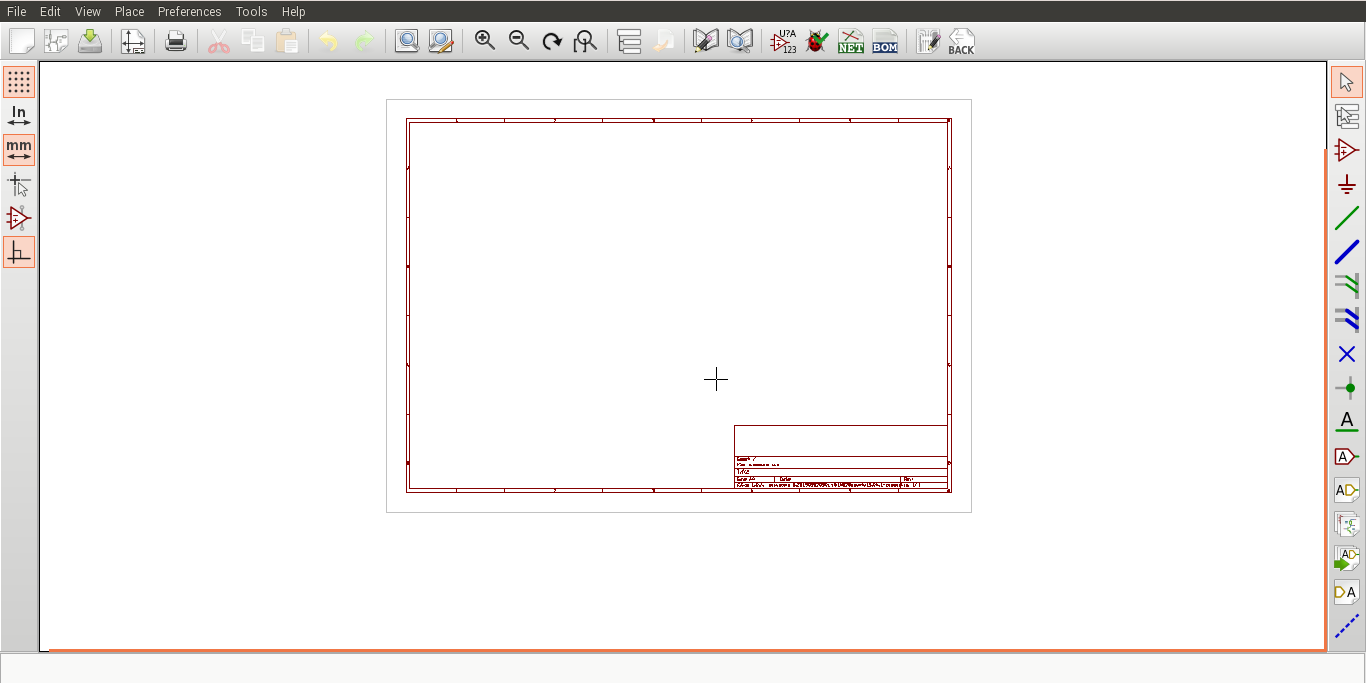
\includegraphics[width=0.5\textwidth, height=6cm]{kicad.png}
\caption{The Kicad Eeschema page}
\label{kicad}
\end{figure}




\begin{figure}[H]
\begin{minipage}{.5\textwidth}
  \centering
  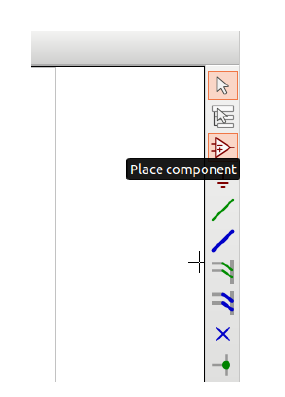
\includegraphics[width=\linewidth]{placecomponent.png}
  \caption{Place component icon}
  \label{placecomponent}
\end{minipage}%
\begin{minipage}{.5\textwidth}
  \centering
  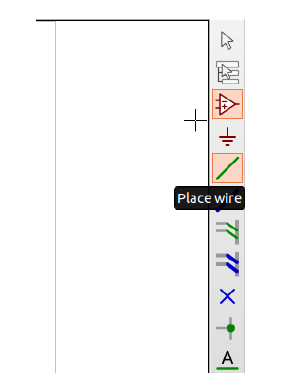
\includegraphics[width=\linewidth]{placewire.png}
  \caption{Place wire icon}
  \label{placewire}
\end{minipage}
\end{figure}


\paragraph{Placing the Components:} Normally all the components availbale in eSim can be chosen by left mouse click in the grid. The components are listed in different libraries. See Figure \ref{librarylist}.

\begin{figure}[H]
\centering
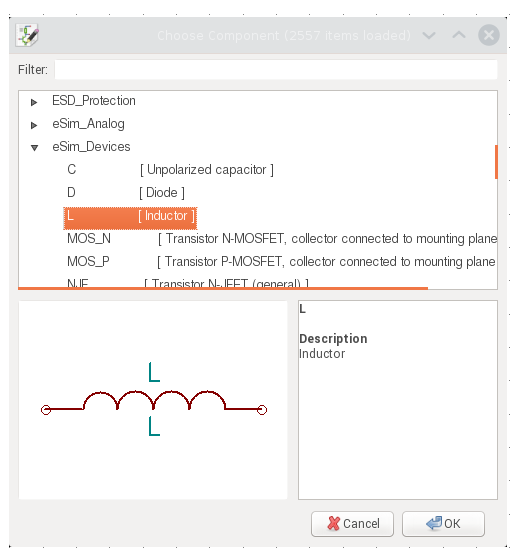
\includegraphics[width=0.5\textwidth, height=4cm]{librarylist.png}
\caption{The Kicad Libraries of components}
\label{librarylist}
\end{figure}

\begin{itemize}
\item
Choose DC source from eSim\_Sources
\item
Choose R from eSim\_Devices
\item
Choose zener from eSim\_Devices
\item
Choose NPN from eSim\_Devices
\item
Choose plot\_v1 from eSim\_Plot

\item
Choose GND from power
\end{itemize}

Select the resistor and edit its component value to 1k as shown in Figure \ref{editvalue}.

\begin{figure}[H]
\centering
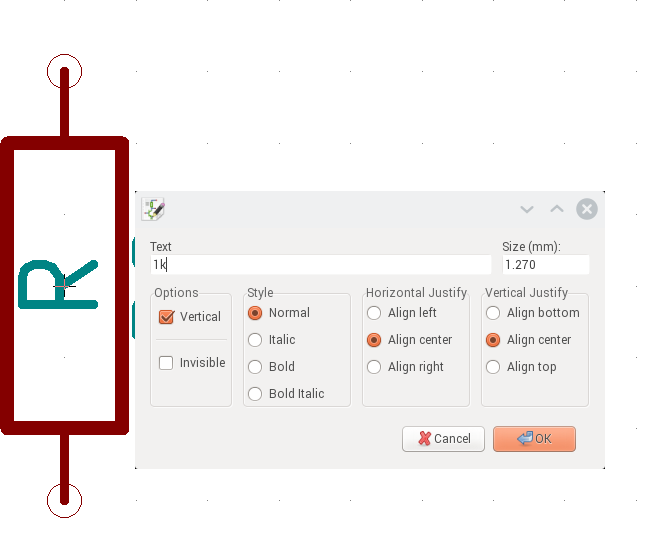
\includegraphics[width=0.5\textwidth, height=6cm]{editvalue.png}
\caption{Editing the value field of component R}
\label{editvalue}
\end{figure}

Wire the components to get the circuit. A global label `in' and `out' has been added to identify that node whose voltage will be later recorded and plotted.

\paragraph{Annotating the circuit:} Once the schematic diagram is completed, annotate it so that the `question marks' associated with the components are converted to meaningful numbers automatically.For that choose annotate button from the top toolbar(See Figure \ref{toptoolbar} and in the subsequenct dialogue boxes appearing click ok and finally close. See Figure \ref{annotation}.

\begin{figure}[H]
\centering
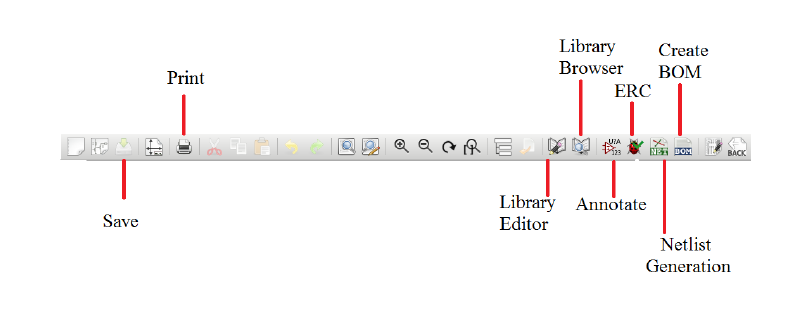
\includegraphics[width=\textwidth, height=4cm]{toptoolbar.png}
\caption{Choose annotate from the toop tool bar}
\label{toptoolbar}
\end{figure}



Now we have the circuit diagram as shown in Figure \ref{zenerregulatorckt}.
\begin{figure}[]
\centering
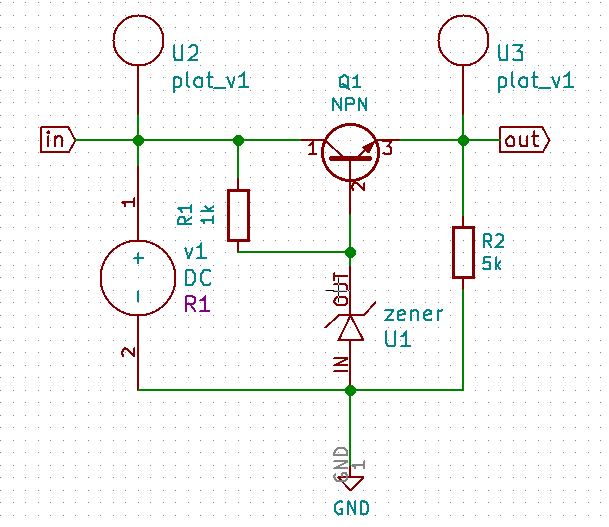
\includegraphics[width=0.8\textwidth]{zenerregulatorckt.png}
\caption{Schematic diagram for Zener Diode Regulator}
\label{zenerregulatorckt}
\end{figure}

\paragraph{Note:} If some libraries are found missing, you can add them from the `Preferences` menu by following the procedure: 

\begin{enumerate}
\item
Choose `Component Libraries' from Preferences menu.

\item
Click on the Add button on the top right side of the window.

\item
Choose the required libraries from `user/share/kicad/library' and click OK button

\end{enumerate}

\subsubsection{Create Netlist}

\paragraph{}To simulate the circuit that has been created in the previous section, we need to generate
its netlist. Netlist is a list of components in the schematic along with their connection
information. To do so, click on the Generate netlist tool from the top toolbar. Click on
spice from the window that opens up. Check the option Default Format. Then click
on Generate. Save the netlist. This will be a *.cir file. Do
not change the directory while saving.See Figure \ref{createnetlist}.
 Now the netlist is ready to be simulated. 
\begin{figure}
\begin{minipage}{.5\textwidth}
  \centering
  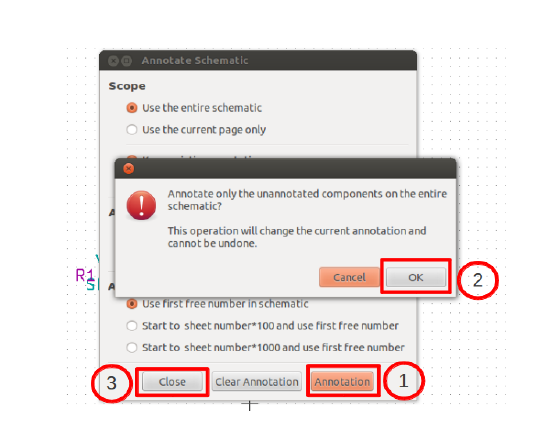
\includegraphics[width=\linewidth]{annotation.png}
  \caption{Annotation}
  \label{annotation}
\end{minipage}%
\begin{minipage}{.5\textwidth}
  \centering
  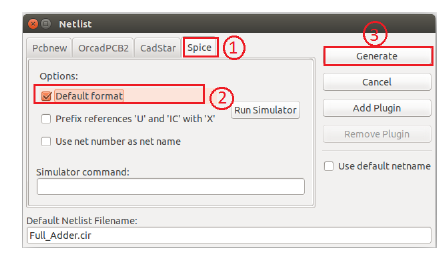
\includegraphics[width=\linewidth]{createnetlist.png}
  \caption{Netlist Generation}
  \label{createnetlist}
\end{minipage}
\end{figure}

\subsubsection{KiCad to Ngspice conversion}

\paragraph{} To convert KiCad netlist of the circuit to NgSpice
compatible netlist click on KiCad to Ngspice icon as shown in Figure \ref{kcd2spice}.  Now you can choose the type of analysis, source details, device models ngspice models and subcircuit models.


\begin{figure}[H]
\centering
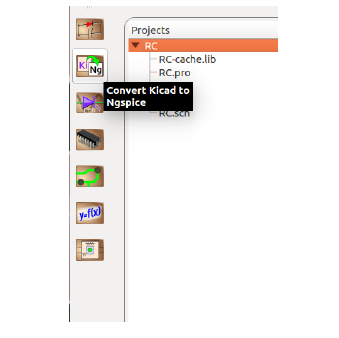
\includegraphics[width=0.5\textwidth, height=4cm]{kcd2spice.png}
\caption{Choose Kicad to Ngspice tool}
\label{kcd2spice}
\end{figure}


\paragraph{Analysis:}Choose DC analysis type. Give the values of DC variables as shown in Figure \ref{zenerregulatorngspice1}. Enter the name of your DC source as on the circuit (here v1) and let its value be varied from 6V to +15V with a step of 1 V.

\begin{figure}[H]
\centering
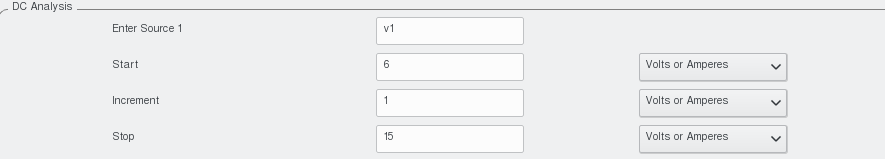
\includegraphics[width=\textwidth, height=4cm]{zenerregulatorngspice1.png}
\caption{Choose DC analysis type and enter the values}
\label{zenerregulatorngspice1}
\end{figure}

\paragraph{Source Details:} Leave this empty.

\paragraph{Ngspice Model:} Ngspice model of zener diode will be loaded. You can see the default values of various zener parameters there. You can change those if required. In this example the breakdown voltage has been set as 8V. See Figure.\ref{zenerregulatorngspice2}
\begin{figure}[H]
\centering
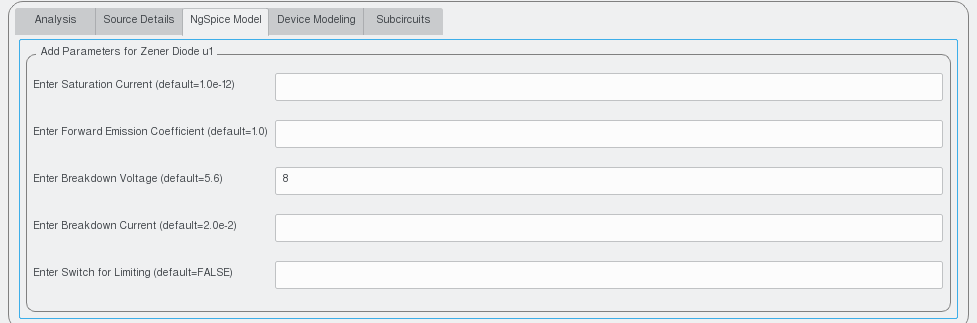
\includegraphics[width=\textwidth, height=4cm]{zenerregulatorngspice2.png}
\caption{Choose ngspice model values}
\label{zenerregulatorngspice2}
\end{figure}

\paragraph{Device Model:} The NPN Transistor is a device whose model details must be given for simulation. Let us choose the generic BJT model availabe in the eSim model library. Browse it from \texttt{/opt/eSim/src/deviceModelLibrary/Transistor/NPN.lib}. See Figure \ref{NPNmodel}.
\begin{figure}[H]
\centering
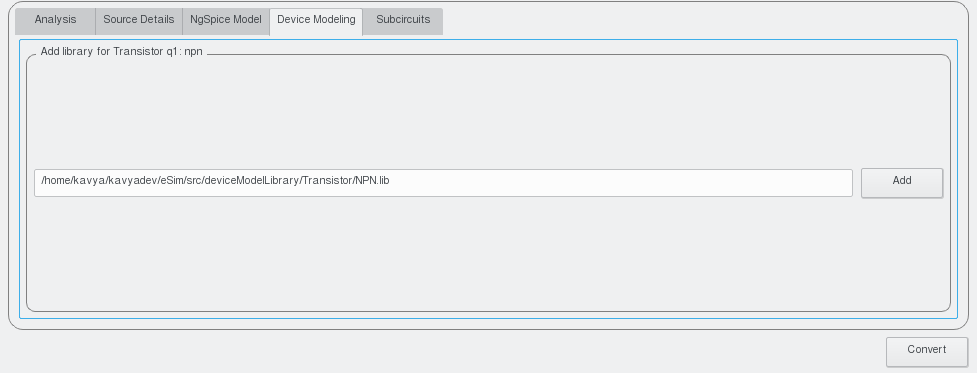
\includegraphics[width=\textwidth, height=6cm]{NPNmodel.png}
\caption{Choose the required Transistor model}
\label{NPNmodel}
\end{figure}

\paragraph{Subcircuits:} No subcircuits to be given.

\noindent Once these details are provided click on convert button. See Figure \ref{NPNmodel}. Now you are ready to see the simulation results.

\subsubsection{Simulate} To run Ngspice simulation click the simulation icon in the left tool bar. It will open up two windows - ngspice plotting window and python plotting window. Inorder to plot the voltages at input and output let us use the commands in ngspice plotting window.

Since we have used \texttt{eSim\_plot} components at \texttt{in} and \texttt{out}, simulate button click will automatically plot the voltages.

\paragraph{}To plot the value of voltages on a signle plot window type the following command 

\texttt{plot v(in), v(out)}

This would pop up the required characteristics fo the diode as defined in the diode model D.lib. For a differnt diode model the characteristics would be slightly different.

The resultant characteristics is shown in the Figure \ref{zenerregulatorchara}.

\begin{figure}[H]
\centering
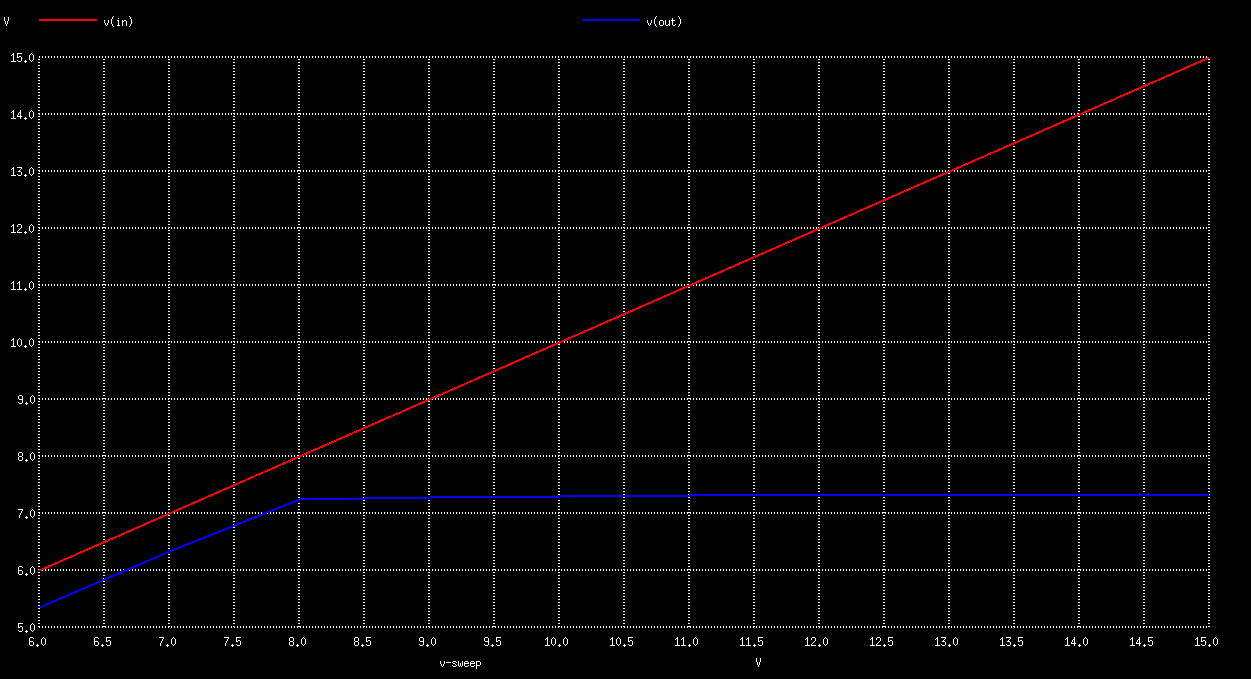
\includegraphics[width=12cm, height=6cm]{zenerregulatorchara.png}
\caption{The line regulation characteristics of zener diode}
\label{zenerregulatorchara}
\end{figure}

\section*{RESULT}
The circuit for plotting the charateristics of zener regulator was implemented and simulated.


